% \setchapterpreamble[u]{\margintoc}
\chapter{Models of type theory}
\labch{models}

Justifying a logic is often achieved using \emph{models}. A model consists
in giving an interpretation to all constructs of the logic we want to study,
such that its rules are still verified.
There are several ways to get models of type theory, I will present some of the
most common ones in this chapter, though my means of choice will presented in
depth in \nrefch{translations}.

\section{What is a model?}

A model of type theory is an interpretation of the concepts of a type theory
into another theory or object, both living in the same meta-theory.
\begin{figure}[hb]
  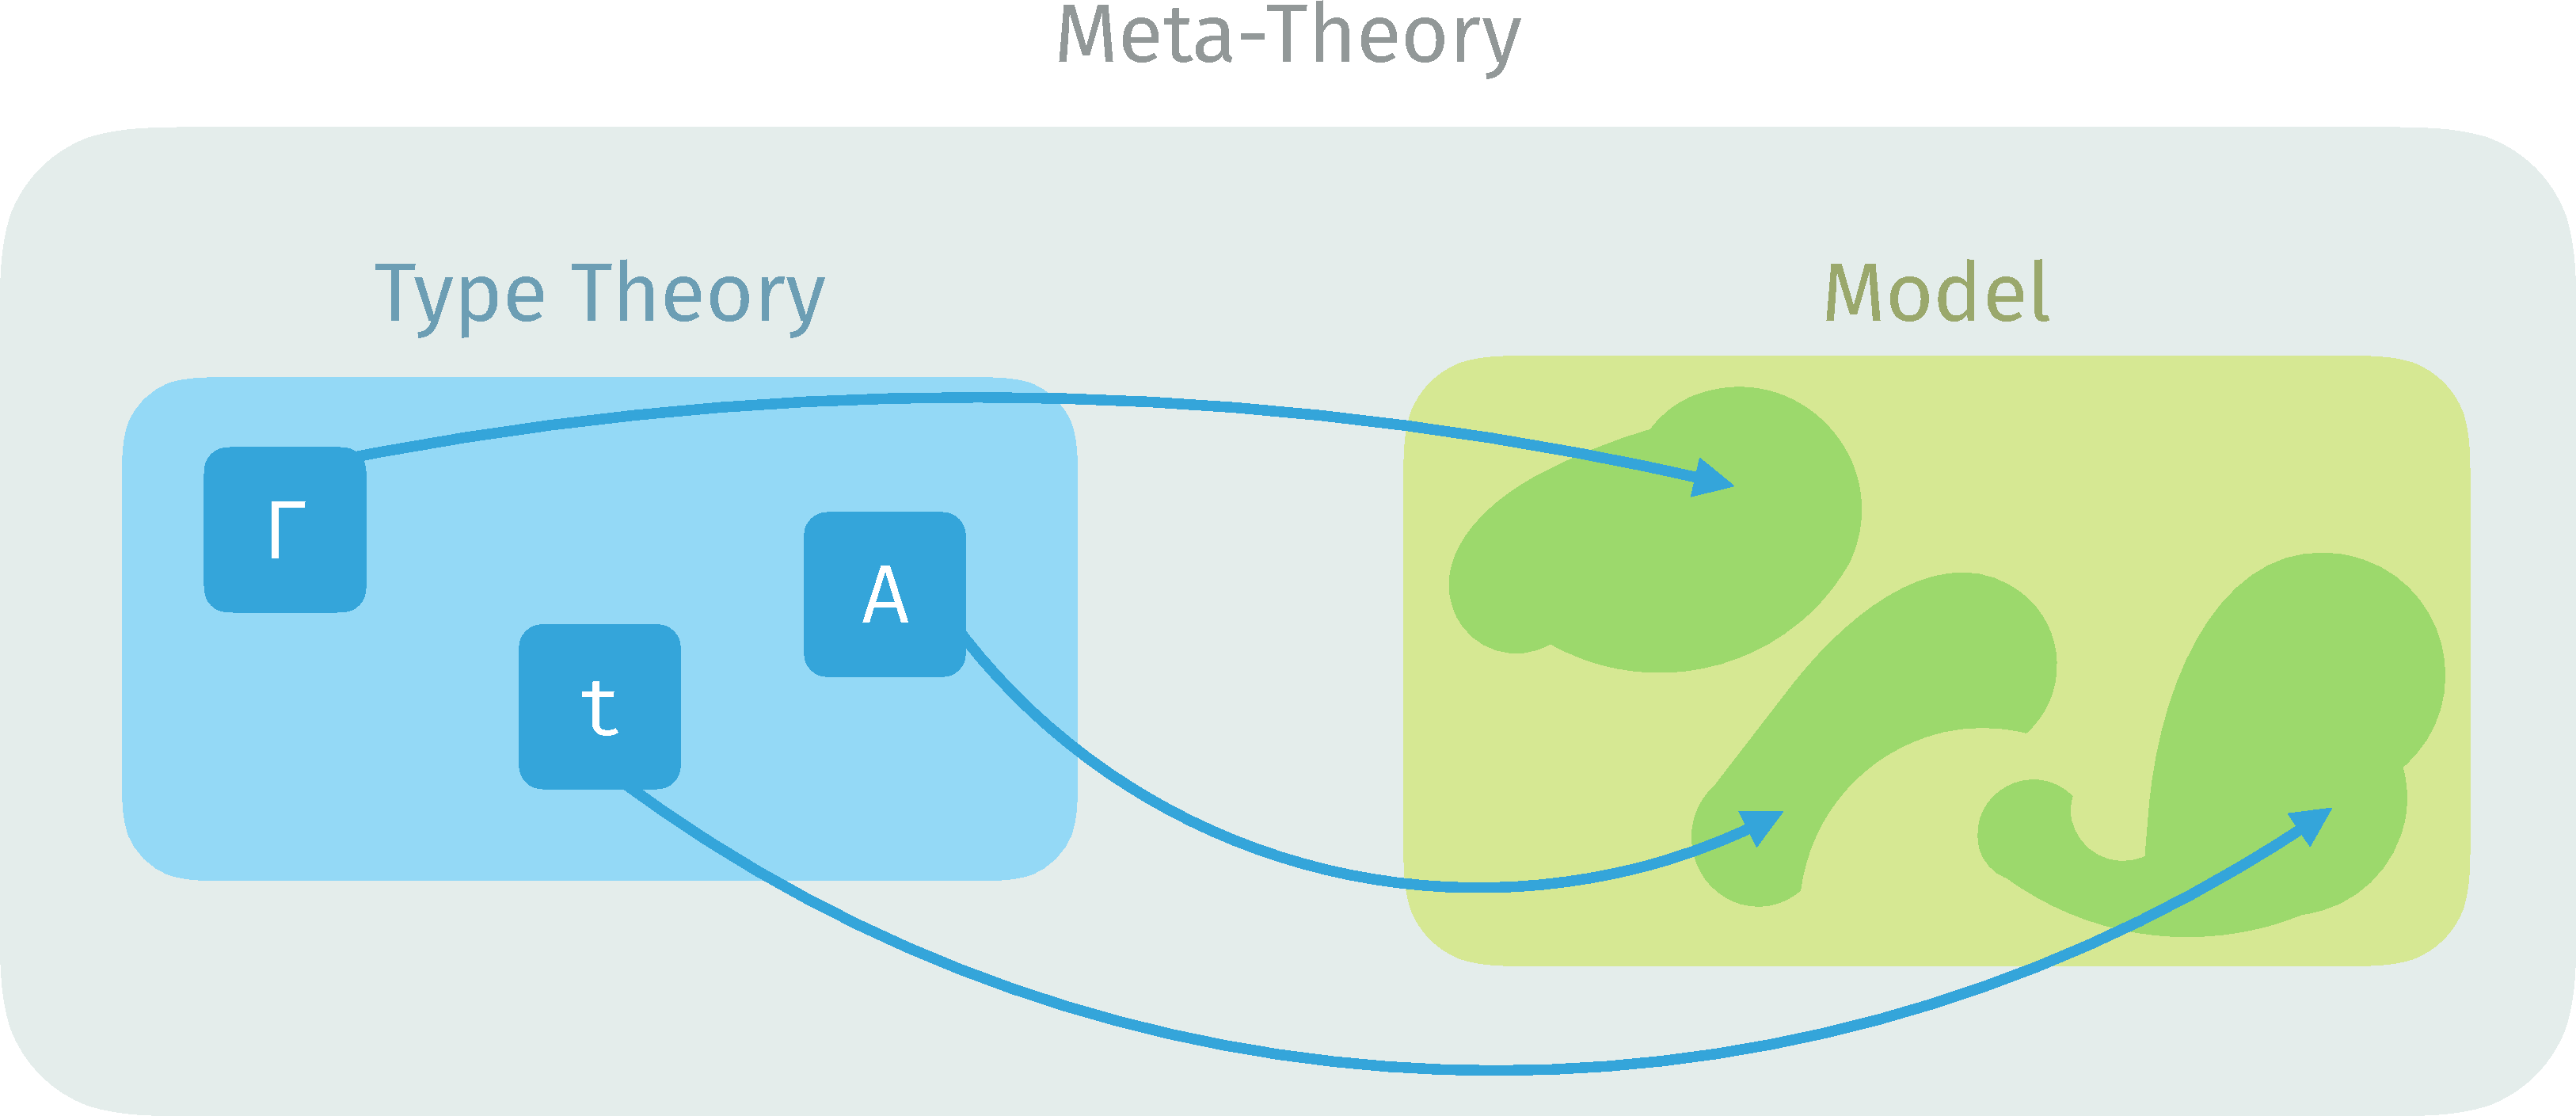
\includegraphics[width=0.9\textwidth]{model}
\end{figure}
To be more precise, a model is given by a class of objects to interpret
contexts, one for terms and one for types; but a model also provides an
interpretation to judgments in such a way that the interpretation is coherent.

\subsection{What can be proved using models}

\paragraph{Consistency.}

I already briefly mentioned this but the main point of models is to prove
consistency of a theory, relying on the already \emph{known} consistency of the
theory in which lives the model... At least in principle. It is however very
rare\sidenote{Impossible?} to \emph{know} that a theory is consistent, instead
we should see it as a theory we \emph{trust}, typically a theory that's widely
accepted as beeing consistent by the community of mathematicians.
This also applies to the meta-theory in which we show that the interpretation is
correct. As such it is best to keep it as simple as possible to avoid relying on
the consistency of too complicated objects.

\paragraph{Independence.}

Another interesing application of models is showing \emph{independence} of a
proposition.

\begin{definition}[Independent proposition]
  A proposition \(P\) is said to be independent from a theory \cT when neither
  \(P\) nor \(\neg P\) can be proven within \cT.
\end{definition}

A way to prove that some \(P\) is independent from \cT is to give a model of \cT
which validates \(P\) and another model which invalidates it (or validates
\(\neg P\)). Indeed if any one of \(P\) or \(\neg P\) %, let's say \(P\),
could be proven in \cT, then it would be valid in both models, leading to
at least one of them being inconsistent.

The fact that a proposition can neither be validated or invalidated in a theory
can come as surprising for some, especially in a classical mindset.
\reminder[-1.8cm]{Classical logic}{
  Classical logic is often characterised by the presence of the \acrshort{LEM}
  which consists in a proof of \(A \vee \neg A\).
}
Gödel's incompleteness theorems have to do with this.

\subsection{Gödel's incompleteness theorems}

\todo{Is it really the place? Should it even go in the proof theory chapter?}

\section{Set-theoretic models}

Set-theoretic models are models of type-theory where types are interpreted as
sets. For instance the type \(A \to B\) will be interpreted as the set of
set-theoretic functions from the interpretation of \(A\) to the interpretation
of \(B\):
\marginnote[0.2cm]{
  It is usual to write \(\transl{A}\) for the interpretation of \(A\).
}
\[
  \transl{A \to B} \coloneqq \setfun{\transl{A}}{\transl{B}})
\]
\todo{I'm missing a ref here on how to do this...}

\section{Categorical models}

Categorical models are one of the most used way of defining models for type
theories. There are several notions of categorical models:
contextual categories~\sidecite[-0.9cm]{cartmell1986generalised} from which stem
categories with attributes~\sidecite[0.2cm]{hofmann1994interpretation} and
C-systems~\sidecite[0.9cm]{voevodsky2016subsystems},
\acrfullpl{CwF}~\sidecite[1.7cm]{dybjer1995internal}, and more\dots
I will focus on \acrshortpl{CwF} in this document.

\subsection{Categories with families}

A \acrshort{CwF} is given by
\begin{enumerate}
  \item a collection of objects (or contexts) \(\Con\);
  \item morphisms (or substitutions) \(\sigma : \Ga \to \D\) between contexts
  \(\Ga, \D : \Con\);
  \item for each context \(\Ga : \Con\), a collection \(\CTy\ \Ga\) of types in
  that context;
  \item for each context \(\Ga : \Con\) and type \(A : \CTy\ \Ga\), a collection
  \(\CTm\ \Ga\ A\) of terms of type \(A\);
  \item an operation of substitution for types taking \(\sigma : \Ga \to \D\)
  and a type \(A : \CTy\ \D\) to type \(A[\sigma] : \CTy\ \Ga\);
  \item \label{item:term-subst} a similar substitution operation on terms taking
  \(\sigma : \Ga \to \D\) and a term \(t : \CTm\ \D\ A\) to term
  \(t[\sigma] : \CTm\ \Ga\ A[\sigma]\);
  \item a terminal object representing the empty context \(\ctxempty : \Con\);
  \item an extension operation taking \(\Ga : \Con\) and \(A : \CTy\ \Ga\)
  to a new object \(\Ga, A : \Con\) together with a morphism
  \(\pp : \Ga, A \to \Ga\) and a term \(\pq : \CTm\ (\Ga, A)\ A[\pp]\);
  \item an operation taking \(\sigma : \Ga \to \D\) and term
  \(a : \CTm\ \Ga\ A[\sigma]\) to substitution \(\sigma, a : \Ga \to \D, A\)
  such that \(\pp \circ (\sigma, a) = \sigma\) and \(\pq[\sigma, a] = a\).
\end{enumerate}
The two first have to give the structure of category, this in particular means
that there is an identity substitution, and associative composition of those.

The category \(\Set\) of sets is a \acrshort{CwF}:
\marginnote[3.8cm]{
  \ref{item:term-subst} holds because for every \(\gamma \in \Ga\),
  \[
    (t \circ \sigma)(\gamma) = t(\sigma(\gamma)) \in A_{\sigma(\gamma)}
    = A[\sigma]_\gamma
  \]
}
\begin{enumerate}
  \item objects are sets;
  \item substitutions are given as set-theoretic functions, composed as
  functions;
  \item types in \(\CTy\ \Ga\) are sets indexed by \(\Ga\);
  \item terms of \(\CTm\ \Ga\ A\) are choice functions
  \(t \in \setfun{\Ga}{\bigcup_{\gamma \in \Ga} A_\gamma}\) such that
  \(t(\gamma) \in A_\gamma\) for every \(\gamma \in \Ga\);
  \item given \(\sigma : \Ga \to \D\) and \(A : \CTy\ \D\), \(A[\sigma]\)
  is defined as the \(\Ga\)-index family \((A_{\sigma(\gamma)})_\gamma\);
  \item given \(\sigma : \Ga \to \D\) and \(t : \CTm\ \D\ A\), \(t[\sigma]\)
  is defined as the choice function \(t \circ \sigma\);
  \item the empty context is given as the singleton \(\{ \emptyset \}\);
  \item given \(\Ga : \Con\) and \(A : \CTy\ \Ga\), \(\Ga, A\) is defined as
  the disjoint union \(\amalg_{\gamma \in \Ga} A_\gamma\), \(\pp\) and \(\pq\)
  are defined as the first and second projection respectively;
  \item given \(\sigma : \Ga \to \D\) and \(a : \CTm\ \Ga\ A[\sigma]\),
  \(\sigma, a\) is defined as the function
  \(\gamma \mapsto (\sigma(\gamma), a(\gamma))\) which verifies the conditions.
\end{enumerate}

Right now this only interprets a type theory with no type or term constructors.
I will give a few example of those.

\paradot{Dependent products}

A \acrshort{CwF} is said to have dependent products when it has the following
elements:
\begin{itemize}
  \item for any \(A : \CTy\ \Ga\) and \(B : \CTy\ (\Ga, A)\) there exists
  \(\Pi\ A\ B : \CTy\ \Ga\);
  \item for \(b : \CTm\ (\Ga, A)\ B\) there exists
  \(\lambda b : \CTm\ \Ga\ (\Pi\ A\ B)\);
  \item for \(f : \CTm\ \Ga\ (\Pi\ A\ B)\) and \(u : \CTm\ \Ga\ A\) there exists
  \(\capp(f,u) : \CTm\ \Ga\ B[\cid, u]\)
\end{itemize}
such that for any \(\sigma : \D \to \Ga\) and terms and types as above the
following equations hold:
\[
  \begin{array}{rcl}
    (\Pi\ A\ B)[\sigma] &=& \Pi\ A[\sigma]\ B[(\sigma \circ \pp), \pq] \\
    (\lambda b)[\sigma] &=& \lambda b[(\sigma \circ \pp), \pq] \\
    (\capp(f,u))[\sigma] &=& \capp(f[\sigma],u[\sigma]) \\
    \capp(\lambda b, u) &=& b[\cid, u] \\
    \lambda \capp(f \circ \pp, \pq) &=& f
  \end{array}
\]

\sidedef[-0.7cm]{\(\eta\)-expansion}{
  \(\eta\)-expansion is defined as follows
  \[
    t \red_\eta \lambda x.\ t\ x
  \]
  \(\eta\)-contraction is the opposite relation.
}
The four first equations are simply there to attest to the good behaviour of
substitution. The last two are more interesting, corresponding to
\(\beta\)-reduction and \(\eta\)-contraction respectively.

\paradot{Dependent sums}

A \acrshort{CwF} has (negative\sidenote{See \nrefch{flavours}.}) dependent sums
when:
\begin{itemize}
  \item for any \(A : \CTy\ \Ga\) and \(B : \CTy\ (\Ga, A)\) there exists
  \(\Sigma\ A\ B : \CTy\ \Ga\);
  \item for \(a : \CTm\ \Ga\ A\) and \(b : \CTm\ \Ga\ B[\cid,a]\) there exists
  the dependent pair \(\dpair{a,b} : \CTm\ \Ga\ (\Sigma\ A\ B)\);
  \item for \(p : \CTm\ \Ga\ (\Sigma\ A\ B)\) there exists
  \(p.1 : \CTm\ \Ga\ A\);
  \item for \(p : \CTm\ \Ga\ (\Sigma\ A\ B)\) there exists
  \(p.2 : \CTm\ \Ga\ B[\cid, p.1]\)
\end{itemize}
such that
\[
  \begin{array}{rcl}
    (\Sigma\ A\ B)[\sigma] &=& \Sigma\ A[\sigma]\ B[(\sigma \circ \pp), \pq] \\
    \dpair{a,b}[\sigma] &=& \dpair{a[\sigma], b[\sigma]} \\
    (p.1)[\sigma] &=& p[\sigma].1 \\
    (p.2)[\sigma] &=& p[\sigma].2 \\
    \dpair{a,b}.1 &=& a \\
    \dpair{a,b}.2 &=& b
  \end{array}
\]

\paradot{Identity types}

A \acrshort{CwF} has identity types---another name for the equality type---when:
\begin{itemize}
  \item for \(A : \CTy\ \Ga\) and \(u, v : \CTm\ \Ga\ A\) there exists
  \(\CId_A\ u\ v : \CTy\ \Ga\);
  \item for \(A : \CTy\ \Ga\) and \(u : \CTm\ \Ga\ A\) there exists
  \(\crefl_u : \CTm\ \Ga\ (\CId_A\ u\ u)\)
\end{itemize}
such that
\[
  \begin{array}{rcl}
    (\CId_A\ u\ v)[\sigma] &=& \CId_{A[\sigma]}\ u[\sigma]\ v[\sigma] \\
    (\crefl_a)[\sigma] &=& \crefl_{a[\sigma]}
  \end{array}
\]
In a lot of models, equality end up being interpreted as the equality of the
model meaning the eliminator is not necessary, hence my not requiring it.

\paradot{Booleans}

A \acrshort{CwF} has booleans when for any \(\Ga : \Con\) it has
\begin{itemize}
  \item \(\bool : \CTy\ \Ga\);
  \item \(\ttrue : \CTm\ \Ga\ \bool\);
  \item \(\ffalse : \CTm\ \Ga\ \bool\);
  \item given \(b : \CTm\ \Ga\ \bool\), \(C : \CTy\ (\Ga, \bool)\),
  \(t : \CTm\ \Ga\ C[\cid, \ttrue]\) and \(f : \CTm\ \Ga\ C[\cid, \ffalse]\),
  some \(\tif{b}{C}{t}{f} : \CTm\ \Ga\ C[\cid, b]\)
\end{itemize}
such that
\[
  \begin{array}{rcl}
    \bool[\sigma] &=& \bool \\
    \ttrue[\sigma] &=& \ttrue \\
    \ffalse[\sigma] &=& \ffalse \\
    \left(\fitif{b}{C}{t}{f}\right)[\sigma] &=&
    \fitif{b[\sigma]}{C[(\sigma \circ \pp), \pq]}{t[\sigma]}{f[\sigma]} \\
    \tif{\ttrue}{C}{t}{f} &=& t \\
    \tif{\ffalse}{C}{t}{f} &=& f
  \end{array}
\]

\paradot{Natural numbers}

A \acrshort{CwF} has natural numbers when, given \(\Ga : \Con\), it has
\marginnote[0.1cm]{
  For the successor I use \(\Pi\)-types when I could have instead put things
  in the context. Both are valid and I'm often favorable to the idea that things
  should be kept separate as much as possible, but the reliance on application
  and everything allows us to avoid proving the same things several times,
  especially since manipulating contexts is so tedious with categories.
}
\begin{itemize}
  \item \(\nat : \CTy\ \Ga\);
  \item \(\czero : \CTm\ \Ga\ \nat\);
  \item for \(n : \CTm\ \Ga\ \nat\), \(\csucc\ n : \CTm\ \Ga\ \nat\);
  \item for \(n : \CTm\ \Ga\ \nat\), \(C : \CTy\ (\Ga, \nat)\),
  \(z : \CTm\ \Ga\ C[\cid, \czero]\) and
  \(s : \CTm\ \Ga\ (\Pi\ \nat\ \Pi\ C\ C[(\pp, \csucc\ \pq) \circ \pp])\),
  there exists \(\natrec_C\ n\ z\ s : \CTm\ \Ga\ C[\cid, n]\)
\end{itemize}
such that
\[
  \begin{array}{rcl}
    \nat[\sigma] &=& \nat \\
    \czero[\sigma] &=& \czero \\
    (\csucc\ n)[\sigma] &=& \csucc\ n[\sigma] \\
    (\natrec_C\ n\ z\ s) &=&
    \natrec_{C[(\sigma \circ \pp), \pq]}\ n[\sigma]\ z[\sigma]\ s[\sigma] \\
    \natrec_C\ \czero\ z\ s &=& z \\
    \natrec_C\ (\csucc\ n)\ z\ s &=& \capp(\capp(s,n), \natrec_C\ n\ z\ s)
  \end{array}
\]

\paradot{Tarski universes}

A Tarski universe is given by
\begin{itemize}
  \item a type \(\CU : \CTy\ \Ga\);
  \item for \(a : \CTm\ \Ga\ \CU\), a type \(\CEl(a) : \CTy\ \Ga\);
  \item for \(a : \CTm\ \Ga\ \CU\), \(b : \CTm\ \Ga\ (\Pi\ \CEl(a)\ \CU)\),
  a term \(\pi(a,b) : \CTm\ \Ga\ \CU\)
\end{itemize}
such that
\[
  \begin{array}{rcl}
    \CU[\sigma] &=& \CU \\
    \CEl(a)[\sigma] &=& \CEl(a[\sigma]) \\
    \CEl(\pi(a,b)) &=& \Pi\ \CEl(a)\ \CEl(\capp(b[\pp], \pq))
  \end{array}
\]
This makes the universe closed under dependent types, we can of course extend
this notion to include other constructions.

All of these can be defined in the \(\Set\) model above. They are however all
simpler cases than the \(\Card\) model I will give in the next section so I
won't detail them.

\subsection{Cardinal model}

In the previous section I briefly presented the \(\Set\) model. Here I will
detail the cardinal model of type theory that we initially wrote with Andrej
Bauer. It teaches us interesting things about syntax and especially about
\acrshort{ETT}.

For every set \(X\) there is a unique cardinal \(\card{X}\) such that
\(X \cong \card{X}\). We choose a bijection \(\beta_X : \setfun{X}{\card{X}}\).
I will write \(\beta\) for \(\beta_X\) when the \(X\) is understood.

The \(\Card\) \acrshort{CwF} is defined very similarly to \(\Set\):
\begin{enumerate}
  \item objects are cardinals;
  \item substitutions are given as set-theoretic functions, composed as
  functions;
  \item types in \(\CTy\ \Ga\) are cardinals indexed by \(\Ga\);
  \item terms of \(\CTm\ \Ga\ A\) are choice functions
  \(t \in \setfun{\Ga}{\bigcup_{\gamma \in \Ga} A_\gamma}\) such that
  \(t(\gamma) \in A_\gamma\) for every \(\gamma \in \Ga\);
  \item given \(\sigma : \Ga \to \D\) and \(A : \CTy\ \D\), \(A[\sigma]\)
  is defined as the \(\Ga\)-index family \((A_{\sigma(\gamma)})_\gamma\);
  \item given \(\sigma : \Ga \to \D\) and \(t : \CTm\ \D\ A\), \(t[\sigma]\)
  is defined as the choice function \(t \circ \sigma\);
  \item the empty context is given as the cardinal \(1\);
  \item given \(\Ga : \Con\) and \(A : \CTy\ \Ga\), \(\Ga, A\) is defined as
  the cardinal of the disjoint union
  \(\card{\amalg_{\gamma \in \Ga} A_\gamma}\), \(\pp\) is defined as
  \(\pi_1 \circ \beta^{-1}\) where \(\pi_1\) is the first projection of the
  disjoint union, \(\pq\) is defined as \(\pi_2 \circ \beta^{-1}\);
  \item given \(\sigma : \Ga \to \D\) and \(a : \CTm\ \Ga\ A[\sigma]\),
  \(\sigma, a\) is defined as the function
  \(\gamma \mapsto \beta(\sigma(\gamma), a(\gamma))\).
\end{enumerate}

Let us verify the coherence conditions:
\[
  \begin{array}{rcl}
    \pp \circ (\sigma, a) &=& \sigma \\
    \pq [\sigma, a] &=& a
  \end{array}
\]
\marginnote[0.8cm]{
  Notice how I verify equality of functions extensionally, that is because we
  are considering set-theoretic functions here.
}
Given \(\sigma : \Ga \to \D\), \(a : \CTm\ \Ga\ A[\sigma]\) and
\(\gamma \in \Ga\) we have
\[
  \begin{array}{lclcl}
    (\pp \circ (\sigma, a))(\gamma) &=&
    \pp((\sigma, a)(\gamma)) \\
    &=& \pp(\beta(\sigma(\gamma),a(\gamma))) \\
    &=& (\pi_1 \circ \beta^{-1})(\beta(\sigma(\gamma),a(\gamma))) \\
    &=& \pi_1(\beta^{-1}(\beta(\sigma(\gamma),a(\gamma)))) \\
    &=& \pi_1(\sigma(\gamma), a(\gamma)) &=& \sigma(\gamma)
  \end{array}
\]
and
\[
  \begin{array}{lclcl}
    (\pq [\sigma, a])(\gamma) &=&
    (\pq \circ (\sigma, a))(\gamma) \\
    &=& \pq((\sigma,a)(\gamma)) \\
    &=& \pq(\beta(\sigma(\gamma),a(\gamma))) \\
    &=& (\pi_2 \circ \beta^{-1})(\beta(\sigma(\gamma),a(\gamma))) \\
    &=& \pi_2(\beta^{-1}(\beta(\sigma(\gamma),a(\gamma)))) \\
    &=& \pi_2(\sigma(\gamma),a(\gamma)) &=& a(\gamma)
  \end{array}
\]

I will now echo the previous section and show that \(\Card\) admits all the
constructions I introduced then.

\paradot{Dependent products}

\sidedef[-0.7cm]{Dependent product of sets}{
  \(\prod_{x \in A} B(x)\) is defined as the set of functions \(f\) from \(A\)
  to \(\bigcup_{x \in A} B(x)\) such that \(f(x) \in B(x)\).
}
Given \(A : \CTy\ \Ga\) and \(B : \CTy\ (\Ga, A)\) we define
\(\Pi\ A\ B : \CTy\ \Ga\) as
\[
  (\Pi\ A\ B)(\gamma) \coloneqq \card{\prod_{x \in A(\gamma)} B(\beta(\gamma,x))}
\]
We define abstraction and application as follows:
\marginnote[0.7cm]{
  With \(b : \CTm\ (\Ga,A)\ B\), \(f : \CTm\ \Ga\ (\Pi\ A\ B)\) and
  \(u : \CTm\ \Ga\ A\).
}
\[
  \begin{array}{lcl}
    (\lambda b)(\gamma) &\coloneqq& \beta(x \mapsto b(\beta(\gamma,x))) \\
    \capp(f,u)(\gamma) &\coloneqq& \beta^{-1}(f(\gamma))(u(\gamma))
  \end{array}
\]
Now we show
\[
  \begin{array}{rcl}
    (\Pi\ A\ B)[\sigma] &=& \Pi\ A[\sigma]\ B[(\sigma \circ \pp), \pq] \\
    (\lambda b)[\sigma] &=& \lambda b[(\sigma \circ \pp), \pq] \\
    (\capp(f,u))[\sigma] &=& \capp(f[\sigma],u[\sigma]) \\
    \capp(\lambda b, u) &=& b[\cid, u] \\
    \lambda \capp(f \circ \pp, \pq) &=& f
  \end{array}
\]

\[
  \begin{array}{rcl}
    (\Pi\ A[\sigma]\ B[(\sigma \circ \pp), \pq])(\gamma)
    &=& \card{
      \prod_{x \in A[\sigma](\gamma)}
      B[(\sigma \circ \pp), \pq](\beta(\gamma, x))
    } \\
    &=& \card{
      \prod_{x \in A(\sigma(\gamma))}
      B(((\sigma \circ \pp), \pq)(\beta(\gamma, x)))
    } \\
    &=& \card{\prod_{x \in A(\sigma(\gamma))} B(\beta(\sigma(\gamma),x))} \\
    &=& (\Pi\ A\ B)(\sigma(\gamma)) \\
    &=& (\Pi\ A\ B)[\sigma](\gamma) \\
    \\
    (\lambda b[(\sigma \circ \pp), \pq])(\gamma)
    &=& \beta(x \mapsto b[(\sigma \circ \pp), \pq](\beta(\gamma,x))) \\
    &=& \beta(x \mapsto b(((\sigma \circ \pp), \pq)(\beta(\gamma,x)))) \\
    &=& \beta(x \mapsto b(\beta(\sigma(\gamma), x))) \\
    &=& (\lambda b)(\sigma(\gamma)) \\
    &=& (\lambda b)[\sigma](\gamma) \\
    \\
    (\capp(f,u))[\sigma](\gamma)
    &=& \capp(f,u)(\sigma(\gamma)) \\
    &=& \beta^{-1}(f(\sigma(\gamma)))(u(\sigma(\gamma))) \\
    &=& \beta^{-1}(f[\sigma](\gamma))(u[\sigma](\gamma)) \\
    &=& \capp(f[\sigma], u[\sigma])(\gamma) \\
    \\
    \capp(\lambda b, u)(\gamma)
    &=& \beta^{-1}((\lambda b)(\gamma))(u(\gamma)) \\
    &=& \beta^{-1}(\beta(x \mapsto b(\beta(\gamma,x))))(u(\gamma)) \\
    &=& (x \mapsto b(\beta(\gamma,x))(u(\gamma)) \\
    &=& b(\beta(\gamma, u(\gamma)) \\
    &=& b[\cid, u](\gamma) \\
    \\
    (\lambda \capp(f \circ \pp, \pq))(\gamma)
    &=& \beta(x \mapsto \capp(f \circ \pp, \pq)(\beta(\gamma,x))) \\
    &=& \beta(x \mapsto \beta^{-1}((f \circ \pp)(\beta(\gamma,x)))(\pq(\beta(\gamma,x))))) \\
    &=& \beta(x \mapsto \beta^{-1}(f(\gamma))(x))) \\
    &=& \beta(\beta^{-1}(f(\gamma))) \\
    &=& f(\gamma)
  \end{array}
\]
\marginnote[-13.2cm]{
  In the argument of \(B\) what happens is
  \[
    \begin{array}{ll}
      \multicolumn{2}{l}{((\sigma \circ \pp), \pq)(\beta(\gamma, x))} \\
      =& \beta((\sigma \circ \pp)(\beta(\gamma, x)), \pq(\beta(\gamma, x))) \\
      =& \beta((\sigma(\pp(\beta(\gamma, x)))), \pq(\beta(\gamma, x))) \\
      =& \beta((\sigma(\pi_1(\gamma, x))), \pi_2(\gamma, x)) \\
      =& \beta(\sigma(\gamma), x)
    \end{array}
  \]
}


\paradot{Dependent sums}

\(\Card\) has dependent sums, as defined as
\[
  (\Sigma\ A\ B)(\gamma) \coloneqq
  \card{\amalg_{x \in A(\gamma)} B(\beta(\gamma,x))}
\]
with constructors and destructors:
\[
  \begin{array}{lcl}
    \dpair{a,b}(\gamma) &\coloneqq& \beta(a(\gamma), b(\gamma)) \\
    p.1 &\coloneqq& \pi_1 \circ \beta^{-1} \circ p \\
    p.2 &\coloneqq& \pi_2 \circ \beta^{-1} \circ p
  \end{array}
\]

We now show
\[
  \begin{array}{rcl}
    (\Sigma\ A\ B)[\sigma] &=& \Sigma\ A[\sigma]\ B[(\sigma \circ \pp), \pq] \\
    \dpair{a,b}[\sigma] &=& \dpair{a[\sigma], b[\sigma]} \\
    (p.1)[\sigma] &=& p[\sigma].1 \\
    (p.2)[\sigma] &=& p[\sigma].2 \\
    \dpair{a,b}.1 &=& a \\
    \dpair{a,b}.2 &=& b
  \end{array}
\]

\[
  \begin{array}{rcl}
    (\Sigma\ A[\sigma]\ B[(\sigma \circ \pp), \pq])(\gamma)
    &=& \card{\amalg_{x \in A[\sigma](\gamma)} B[(\sigma \circ \pp), \pq](\beta(\gamma,x))} \\
    &=& \card{\amalg_{x \in A(\sigma(\gamma))} B(\beta(\sigma(\gamma), x))} \\
    &=& (\Sigma\ A\ B)(\sigma(\gamma)) \\
    &=& (\Sigma\ A\ B)[\sigma](\gamma) \\
    \\
    \dpair{a[\sigma], b[\sigma]}(\gamma)
    &=& \beta(a(\sigma(\gamma)), b(\sigma(\gamma))) \\
    &=& \dpair{a,b}[\sigma](\gamma) \\
    \\
    (p[\sigma].1)(\gamma)
    &=& \pi_1(\beta^{-1}(p(\sigma(\gamma)))) \\
    &=& (p.1)[\sigma](\gamma) \\
    \\
    (p[\sigma].2)(\gamma)
    &=& \pi_2(\beta^{-1}(p(\sigma(\gamma)))) \\
    &=& (p.2)[\sigma](\gamma) \\
    \\
    (\dpair{a,b}.1)(\gamma)
    &=& \pi_1(\beta^{-1}(\dpair{a,b}(\gamma))) \\
    &=& \pi_1(\beta^{-1}(\beta(a(\gamma), b(\gamma)))) \\
    &=& a(\gamma) \\
    \\
    (\dpair{a,b}.2)(\gamma)
    &=& \pi_2(\beta^{-1}(\dpair{a,b}(\gamma))) \\
    &=& \pi_2(\beta^{-1}(\beta(a(\gamma), b(\gamma)))) \\
    &=& b(\gamma)
  \end{array}
\]

\paradot{Identity types}

Crucially, \(\Card\) has identity types.
Given \(A : \CTy\ \Ga\) and \(u, v : \CTm\ \Ga\ A\), we define
\(\CId_A\ u\ v : \CTy\ \Ga\) to be the type family
\[
  (\CId_A\ u\ v)(\gamma) \coloneqq \{ 0 \mid u(\gamma) = v(\gamma) \}
\]
The set \(\{ 0 \mid u(\gamma) = v(\gamma) \}\) is indeed a cardinal number,
namely \(0\) when \(u(\gamma) \not= v(\gamma)\) and \(1\) when
\(u(\gamma) = v(\gamma)\).
In fact, \(u(\gamma) = v(\gamma)\) is equivalent to
\(0 \in (\CId_A\ u\ v)(\gamma)\).
Thus, we define \(\crefl_u : \CTm\ \Ga\ (\CId_A\ u\ u)\) as
\[
  (\crefl_u)(\gamma) \coloneqq 0
\]
which is the only possible function.

We check
\[
  \begin{array}{rcl}
    (\CId_A\ u\ v)[\sigma] &=& \CId_{A[\sigma]}\ u[\sigma]\ v[\sigma] \\
    (\crefl_a)[\sigma] &=& \crefl_{a[\sigma]}
  \end{array}
\]

\[
  \begin{array}{rcl}
    \CId_{A[\sigma]}\ u[\sigma]\ v[\sigma]
    &=& \{ 0 \mid u[\sigma](\gamma) = v[\sigma](\gamma) \} \\
    &=& \{ 0 \mid u(\sigma(\gamma)) = v(\sigma(\gamma)) \} \\
    &=& (\CId_A\ u\ v)(\sigma(\gamma)) \\
    &=& (\CId_A\ u\ v)[\sigma](\gamma) \\
    \\
    \crefl_{a[\sigma]}(\gamma)
    &=& 0 \\
    &=& (\crefl_a)(\sigma(\gamma)) \\
    &=& (\crefl_a)[\sigma](\gamma)
  \end{array}
\]

Now that we have equality I will why we don't need an eliminator in this
particular case.

\begin{theorem}
  The cardinal model validates equality reflection.
\end{theorem}
\reminder[-1.6cm]{Reflection rule}{
  \begin{equation*}
    \infer[]
      {\isterm{\Ga}{e}{\Eq{A}{u}{v}}}
      {\eqterm{\Ga}{u}{v}{A}}
    %
  \end{equation*}
  See \refdef{reflection}
}%
%
\begin{proof}
  Assuming that we have \(p : \CTm\ \Ga\ (\CId_A\ u\ v)\) we want to show that
  \(u\) and \(v\) are equal choice functions, \ie that \(u(gamma) = v(\gamma)\)
  for all \(\gamma \in \Ga\).
  Because \(0 = p(\gamma) \in (\CId_A\ u\ v)(\gamma)\), it follows that
  \(u(\gamma) = v(\gamma)\).
\end{proof}

The cardinal model is even stronger than that in that it validates isomorphism
reflection.
An isomorphism \(A \cong B\) is given by two functions \(f : A \to B\)
and \(g : B \to A\) that are inverses of each other (for the type-theoretic
equality).

\begin{definition}[Isomorphism reflection]
  Isomorphism reflection states that isomorphic types are \emph{convertible}:
  \[
    \infer
      {\Ga \vdash e : A \cong B}
      {\Ga \vdash A \equiv B}
    %
  \]
\end{definition}

This consists in a strong invariance principle stating that isomorphic types
cannot be distinguished. Another invariance principle is the univalence axiom.

\begin{theorem}
  The cardinal model validates isomorphism reflection.
\end{theorem}

\begin{proof}
  Assume we are given isomorphic type \(A, B : \CTy\ \Ga\), that is two
  functions \(f : \CTm\ \Ga\ (\Pi\ A\ B[\pp])\) and
  \(g : \CTm\ \Ga\ (\Pi\ B\ A[\pp])\) as well as two equalities showing they
  are mutual inverses:
  \[
    \begin{array}{l}
      p :
      \CTm\ \Ga\
      (\Pi\ A\ \CId_{A[\pp]}\ \capp(g[\pp], \capp(f[\pp], \pq))\ \pq) \\
      q :
      \CTm\ \Ga\
      (\Pi\ B\ \CId_{B[\pp]}\ \capp(f[\pp], \capp(g[\pp], \pq))\ \pq)
    \end{array}
  \]

  We want to show equality of \(A\) and \(B\) that is \(A(\gamma) = B(\gamma)\)
  for every \(\gamma \in \Ga\). Given such \(\gamma\), we have
  \(f(\gamma) \in \card{\prod_{x \in A(\gamma)} B[\pp](\beta(\gamma,x))}\)
  which is to say \(f(\gamma) \in \card{\setfun{A(\gamma)}{B(\gamma)}}\),
  similarly \(g(\gamma) \in \card{\setfun{B(\gamma)}{A(\gamma)}}\).
  We thus have two functions
  \[
    \begin{array}{rcl}
      \beta^{-1}(f(\gamma)) &\in& \setfun{A(\gamma)}{B(\gamma)} \\
      \beta^{-1}(g(\gamma)) &\in& \setfun{B(\gamma)}{A(\gamma)}
    \end{array}
  \]
  We show they are in bijection using \(p\) and \(q\):
  \[
    \begin{array}{rcl}
      \beta^{-1}(p(\gamma)) &\in&
      \prod_{a \in A(\gamma)}
      \{ 0 \mid \beta^{-1}(g(\beta^{-1}(f(\gamma)))) = a \} \\
      \beta^{-1}(q(\gamma)) &\in&
      \prod_{b \in B(\gamma)}
      \{ 0 \mid \beta^{-1}(f(\beta^{-1}(g(\gamma)))) = b \}
    \end{array}
  \]
  Since \(A(\gamma)\) and \(B(\gamma)\) are cardinals in bijection, they are
  necessarily equal: \(A(\gamma) = B(\gamma)\).
\end{proof}

\reminder[-0.7cm]{Injectivity of \(\Pi\)-types}{
  Whenever \(\Pi (x:A).B \equiv \Pi (x:A').B'\)
  then we have both \(A \equiv A'\) and \(B \equiv B'\).
}
This means that the cardinal model validates strange equalities like that of
Cantor space and Baire space \(2^{\mathbb{N}} = \mathbb{N}^{\mathbb{N}}\)
which violates injectivity of \(\Pi\)-types.

All this proves that in type theory, one cannot distinguish isomorphic types.

\paradot{Booleans}

\(\Card\) has booleans, defined as
\[
  \begin{array}{rcl}
    \bool(\gamma) &=& 2 \\
    \ttrue(\gamma) &=& 1 \\
    \ffalse(\gamma) &=& 0 \\
    (\tif{b}{C}{t}{f})(\gamma) &=&
    \left\{
    \begin{array}{ll}
      t(\gamma) & \text{if \(b(\gamma) = 1\)} \\
      f(\gamma) & \text{otherwise}
    \end{array}
    \right.
  \end{array}
\]

The equations are
\[
  \begin{array}{rcl}
    \bool[\sigma] &=& \bool \\
    \ttrue[\sigma] &=& \ttrue \\
    \ffalse[\sigma] &=& \ffalse \\
    \left(\fitif{b}{C}{t}{f}\right)[\sigma] &=&
    \fitif{b[\sigma]}{C[(\sigma \circ \pp), \pq]}{t[\sigma]}{f[\sigma]} \\
    \tif{\ttrue}{C}{t}{f} &=& t \\
    \tif{\ffalse}{C}{t}{f} &=& f
  \end{array}
\]

The first three hold trivially. I prove the remaining below.
\[
  \begin{array}{rcl}
    \left(
      \fitif{b[\sigma]}{C[(\sigma \circ \pp), \pq]}{t[\sigma]}{f[\sigma]}
    \right)(\gamma)
    &=&
    \left\{
    \begin{array}{ll}
      t(\sigma(\gamma)) & \text{if \(b(\sigma(\gamma)) = 1\)} \\
      f(\sigma(\gamma)) & \text{otherwise}
    \end{array}
    \right. \\
    &=& \left(\fitif{b}{C}{t}{f}\right)[\sigma](\gamma) \\
    \\
    \tif{\ttrue}{C}{t}{f}
    &=&
    \left\{
    \begin{array}{ll}
      t(\gamma) & \text{if \(\ttrue(\gamma) = 1\)} \\
      f(\gamma) & \text{otherwise}
    \end{array}
    \right. \\
    &=& t(\gamma) \\
    \\
    \tif{\ffalse}{C}{t}{f}
    &=&
    \left\{
    \begin{array}{ll}
      t(\gamma) & \text{if \(\ffalse(\gamma) = 1\)} \\
      f(\gamma) & \text{otherwise}
    \end{array}
    \right.\\
    &=& f(\gamma)
  \end{array}
\]

\paradot{Natural numbers}

We define natural numbers as the cardinal of \(\mathbb{N}\):
\[
  \nat(\gamma) \coloneqq \omega
\]
Zero is the constant function
\[
  \czero(\gamma) \coloneqq 0
\]
while the successor of a natural number is defined as
\[
  (\csucc\ n)(\gamma) \coloneqq n(\gamma) + 1
\]
The eliminator is a bit more complex but not too surprising:
% \[
%   (\natrec_C\ n\ z\ s)(\gamma) \coloneqq
%   \left\{
%   \begin{array}{ll}
%     z(\gamma) & \text{when \(n(\gamma) = 0\)} \\
%     \capp(\capp(s, (x \mapsto m)), \natrec_C\ (x \mapsto m)\ z\ s)(\gamma) &
%     \text{when \(n(\gamma) = m + 1\)}
%   \end{array}
%   \right.
% \]
\[
  \begin{array}{l}
    (\natrec_C\ n\ z\ s)(\gamma) \coloneqq
    \left\{
    \begin{array}{ll}
      z(\gamma) & \text{when \(n(\gamma) = 0\)} \\
      f(\gamma) &
      \text{when \(n(\gamma) = m + 1\)}
    \end{array}
    \right. \\
    \text{where } f \coloneqq
    \capp(\capp(s, (x \mapsto m)), \natrec_C\ (x \mapsto m)\ z\ s)
  \end{array}
\]

The equalities are fairly straightforward.
\[
  \begin{array}{rcl}
    \nat[\sigma] &=& \nat \\
    \czero[\sigma] &=& \czero \\
    (\csucc\ n)[\sigma] &=& \csucc\ n[\sigma] \\
    (\natrec_C\ n\ z\ s)[\sigma] &=&
    \natrec_{C[(\sigma \circ \pp), \pq]}\ n[\sigma]\ z[\sigma]\ s[\sigma] \\
    \natrec_C\ \czero\ z\ s &=& z \\
    \natrec_C\ (\csucc\ n)\ z\ s &=& \capp(\capp(s,n), \natrec_C\ n\ z\ s)
  \end{array}
\]

\paradot{Tarski universes}

If \(\kappa\) is an inaccessible cardinal then we get a universe by taking
\[
  \begin{array}{lcl}
    \CU(\gamma) &\coloneqq& \kappa \\
    \CEl(a)(\gamma) &\coloneqq& \card{a(\gamma)} \\
    \pi(a,b)(\gamma) &\coloneqq&
    \prod_{x \in \card{a(\gamma)}} \card{\beta^{-1}(b(\gamma))(x)}
  \end{array}
\]

A perhaps more interesting universe is given by using the \(\aleph\) function:
\[
  \begin{array}{lcl}
    \CU(\gamma) &\coloneqq& \kappa \\
    \CEl(a)(\gamma) &\coloneqq& \aleph_{a(\alpha)} \\
    \pi(a,b) &\coloneqq& \mu
  \end{array}
\]
where
\(\aleph_\mu = \prod_{x \in \CEl{a(\gamma)}} \CEl{\beta^{-1}(b(\gamma))(x)}\).

\section{Type-theoretic models}

\todo{Cat models fall in this too}
\todo{translations, syntactical models, standard model}